\documentclass[8pt]{extarticle}
\title{Econ 250 HW 2}
\author{Avinash Iyer}
\date{September 14, 2022}

%font setup
%
%\usepackage[math]{anttor}

%paper setup
\usepackage{geometry}
\geometry{letterpaper, portrait, margin=1in}
\usepackage{fancyhdr}

%symbols
\usepackage{amsmath}
\usepackage{amssymb}
\usepackage{hyperref}
\usepackage{gensymb}

\usepackage[T1]{fontenc}
\usepackage[utf8]{inputenc}

%chemistry stuff
\usepackage[version=4]{mhchem}
\usepackage{chemfig}

%plotting
\usepackage{pgfplots}
\usepackage{tikz}

%\usepackage{natbib}

%graphics stuff
\usepackage{graphicx}
\graphicspath{ {./images/} }

%a useful command
\newcommand{\plain}[1]{\textrm{#1}}

%code stuff
%when using minted, make sure to add the -shell-escape flag
%you can use lstlisting if you don't want to use minted
%\usepackage{minted}
%\usemintedstyle{pastie}
%\newminted[javacode]{java}{frame=lines,framesep=2mm,linenos=true,fontsize=\footnotesize,tabsize=3,autogobble,}
%\newminted[cppcode]{cpp}{frame=lines,framesep=2mm,linenos=true,fontsize=\footnotesize,tabsize=3,autogobble,}

\usepackage{listings}
\usepackage{color}
\definecolor{dkgreen}{rgb}{0,0.6,0}
\definecolor{gray}{rgb}{0.5,0.5,0.5}
\definecolor{mauve}{rgb}{0.58,0,0.82}

\lstset{frame=tb,
	language=Java,
	aboveskip=3mm,
	belowskip=3mm,
	showstringspaces=false,
	columns=flexible,
	basicstyle={\small\ttfamily},
	numbers=none,
	numberstyle=\tiny\color{gray},
	keywordstyle=\color{blue},
	commentstyle=\color{dkgreen},
	stringstyle=\color{mauve},
	breaklines=true,
	breakatwhitespace=true,
	tabsize=3
}
\pagestyle{fancy}
\fancyhf{}
\rhead{Avinash Iyer}
\lhead{}
\begin{document}{
\maketitle
\section*{Changes in market equilibria}
\subsection*{Part A}
Market Equilibrium Price and Quantity as a function of Income:
\begin{align*}
Q_s &= 1000+P \\
Q_d &= 10000 - 2P - 6I \\
1000+P &= 10000 - 2P - 6I \\
3P &= 9000 - 6I \\
P^{*} &= \boxed{3000-I} \\
\\
Q^{*} &= 1000 + (3000 - I)\\
&= \boxed{4000-I}
\end{align*}
\subsection*{Part B}
Since the derivative of quantity with respect to income $\frac{dQ}{dI} = -1$, this means that as income rises, the quantity demanded will fall. This means that the good in question is an inferior good.
\section*{Elasticities}
Suppose that a typical consumer has an inverse demand for frog legs given by $P = \frac{3}{Q}$.
\subsection*{Part A}
The own price elasticity of demand is given as follows:
\begin{align*}
	P &= \frac{3}{Q}\\
	Q &= \frac{3}{P}\\
	\frac{dQ}{dP} &= -\frac{3}{P^2} \\
	E_{\plain{own}} &= \frac{dQ}{dP}\left(\frac{P}{Q}\right) \\
	&= -\frac{3}{P^2}\left(\frac{P}{\frac{3}{P}}\right)\\
	&= \boxed{-1}
\end{align*}
\subsection*{Part B}
If price increases by 10\%, the quantity demanded will decrease by exactly 10\%. The demand for frog legs is unitary elastic.
\pagebreak
\subsection*{Part C}
\begin{figure}[h]
	\centering
	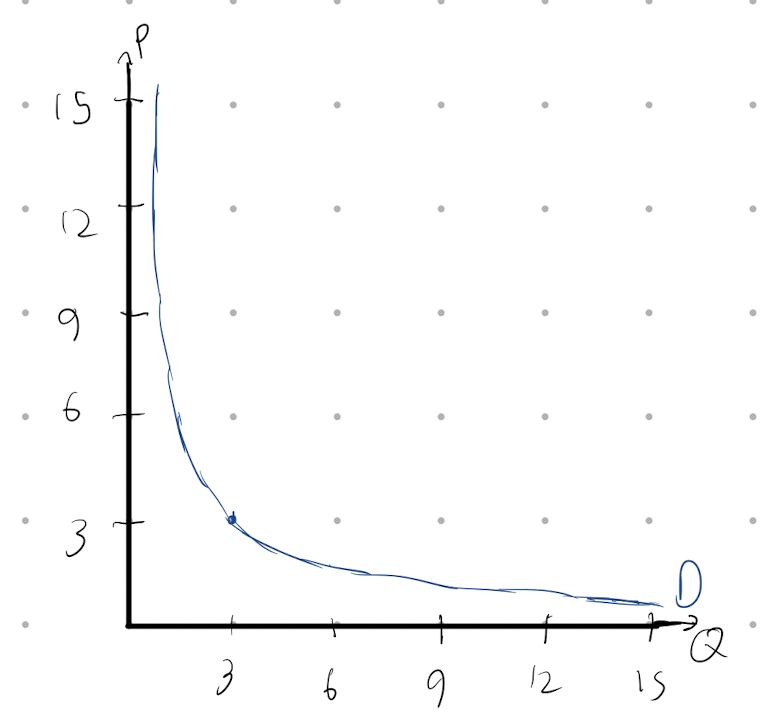
\includegraphics[width=10cm]{HW2Q2C}
\end{figure}
\noindent Because this demand curve has a hyperbolic shape, the elasticity at each point in the curve is the same, namely that it is unitary elastic.
\section*{Elasticities, cont'd}
\subsection*{Part A}
\begin{align*}
	P_G &= \sqrt{\frac{5I}{Q}}\\
	Q &= \frac{5I}{{P_G}^2}\\
	E_{\plain{cross}} &= \frac{dQ}{dP_G}\left(\frac{P_G}{Q}\right)\\
	&= -\frac{5I}{2{P_G}^3}\left(\frac{P_G}{\frac{5I}{{P_G}^2}}\right)\\
	&= \boxed{-\frac{1}{2}}
\end{align*}
The magnitude of the cross price elasticity of demand is less than 1, meaning that lemonade and green tea are complements and that the demand for lemonade is inelastic with respect to a change in the price of green tea.
\subsection*{Part B}
\begin{align*}
	P_G &= \sqrt{\frac{5I}{Q}}\\
	Q &= \frac{5I}{{P_G}^2}\\
	E_{\plain{income}} &= \frac{dQ}{dI}\left(\frac{I}{Q}\right)\\
	&= \frac{5}{{P_G}^2}\left(\frac{I}{\frac{5I}{{P_G}^2}}\right)\\
	&= 1
\end{align*}
The income elasticity of demand for green tea is positive, meaning that it is a normal good.
\section*{Taxes}
\subsection*{Part A}
\begin{align*}
	Q_D &= 1000 - 3P_{c}\\
	Q_S &= 6P_{p} - 800\\
	P_{p} &= P_{c} - 30 \\
	1000 - 3P_c &= 6(P_c-30) - 800\\
	1800+180 &= 9P_{c}\\
	P_{c} &= 220\\
	P_p &= 190\\
	Q_D &= 1000-3(220)\\
	&= \boxed{340}
\end{align*}
\subsection*{Part B}
It is not possible for the government to make the producer and consumer share the tax burden equally because the elasticities of demand and supply are different — the consumer has a more inelastic demand than the producer has supply, so the consumer will bear more of the tax burden.
\section*{Subsidies}
\subsection*{Part A}
\begin{align*}
	Q_{D} &= 30-P\\
	Q_S &= 3P-10 \\
	30-P &= 3P-10\\
	P &= \boxed{10}\\
	Q &= \boxed{20}
\end{align*}
\subsection*{Part B}
\begin{align*}
	Q_D &= 30-P_c\\
	Q_S &= 3P_s-10\\
	P_s &= P_c + 4\\
	30-P_c &= 3(P_c+4)-10\\
	40-12 &= 4P_c\\
	P_c &= \boxed{7}\\
	P_p &= \boxed{11}\\
	Q &= \boxed{23}
\end{align*}
\subsection*{Part C}
75\% of the subsidy is received by consumers (the drop in price they receive is \$3 of the \$4 spent on the subsidy). The producer only receives 25\% of the subsidy, since the demand for quinoa is much more inelastic than the supply of quinoa, so subsidies to purchase quinoa are absorbed by the consumer much more than by the producer.
\subsection*{Part D}
\begin{align*}
	26 &= 30 - P_c\\
	P_c &= 4\\
	26 &= 3P_p - 10\\
	P_p &= 12\\
	S &= P_p - P_c\\
	S &= \boxed{8}
\end{align*}
\section*{Taxes, cont'd}
\begin{align*}
	P &= 40-0.2Q_D\\
	10 &= 40-0.2Q_D\\
	Q_D &= 150\\
	Q_D &= 40-5P_c\\
	P_t &= 40-0.2(Q_D+50) && (\plain{using rules from algebra, shift inverse $D$ curve 50 units left})\\
\end{align*}
The difference between this new demand curve and the existing demand curve is $t= 10$, meaning that the government should put a unit tax of $10$ in order to achieve its desired outcome of $100$ cheesecakes consumed instead of $150$ cheesecakes.
\section*{Elasticities and Tax Incidence}
\subsection*{Part A}
The demand for carrots is much more inelastic than the supply of carrots as 75\% of the tax was absorbed by the consumer.
\subsection*{Part B}
\begin{align*}
	Q_D &= 150 - p\\
	Q_S &= 20 + Mp\\
	150-p &= 20 + Mp\\
	Mp+p &= 130\\
	Q_D &= 150 - (p+1.5)\\
	Q_S &= 20 + M(p-0.5)\\
	150 - p - 1.5 &= 20 + Mp - 0.5M\\
	127.5 &= Mp+p-0.5M\\
	127.5 &= 130 - 0.5M\\
	0.5M &= 2.5\\
	M = \boxed{5}
\end{align*}
\pagebreak
\section*{Elasticities and Tax Incidence, cont'd}
\subsection*{Part A}
\begin{figure}[h]
	\centering
	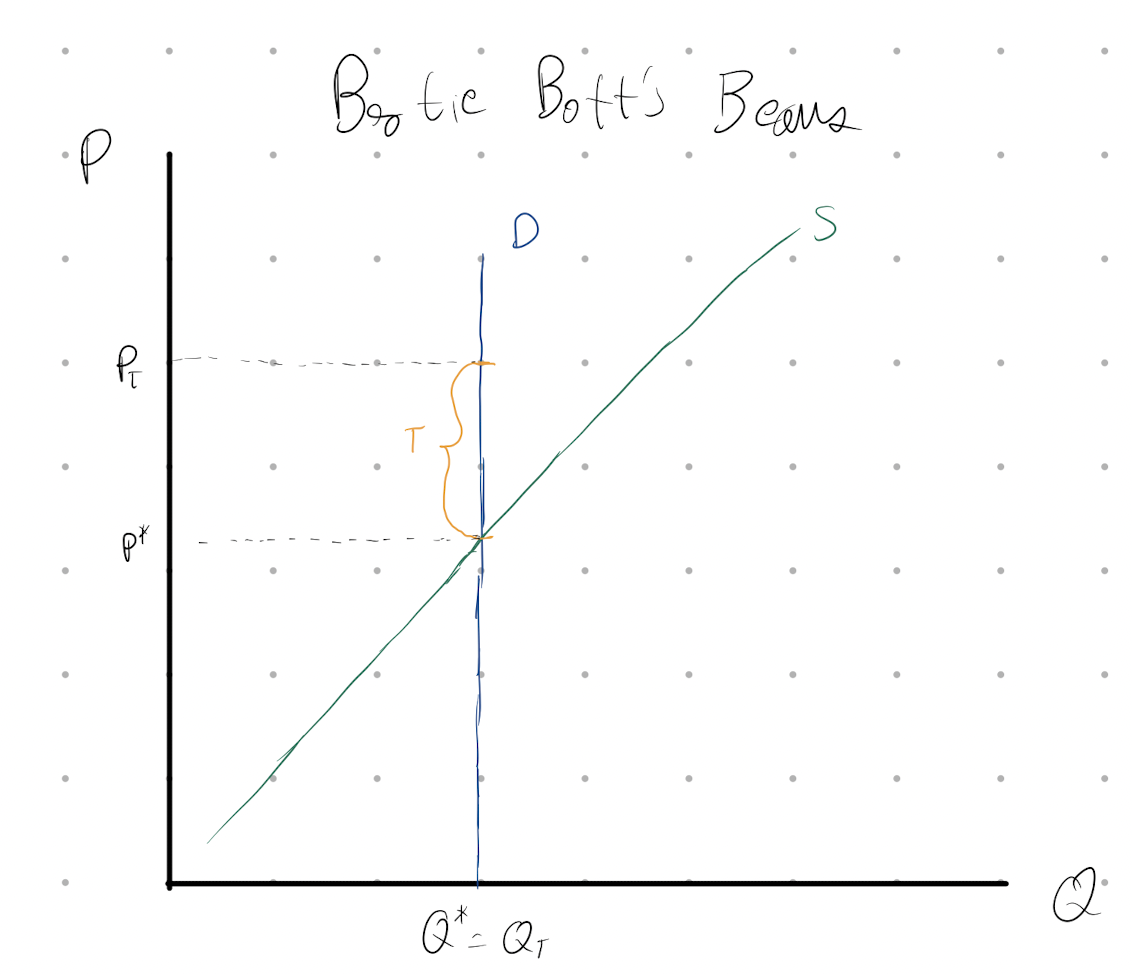
\includegraphics[width=10cm]{HW2Q8A}
\end{figure}
\subsection*{Part B}
Both Parvati and Padma are wrong — because the demand for Bertie Bott's Beans is perfectly inelastic, any tax regardless of whether it is levied on the consumers or producers will have no effect on the amount of beans purchased.
\section*{Elasticities and Tax Incidence, cont'd 2}
\subsection*{Part A}
\begin{align*}
	E_{\plain{own}} &= \frac{dK}{dP_{K}}\left(\frac{P_K}{K}\right)\\
	&= -\frac{15IP_C}{{P_K}^4}\left(\frac{P_K}{\frac{5IP_C}{{P_K}^3}}\right)\\
	&= -3
\end{align*}
\subsection*{Part B}
It is possible to calculate the incidence of the tax on consumers, and from there it is possible to calculate the size of the tax.
\begin{align*}
	\frac{\Delta P_{c}}{T} &= \frac{E_s}{E_s + |E_d|}\\
	\frac{6}{T} &= \frac{2}{2 + 3}\\
	T &= \boxed{15}
\end{align*}
\section*{Preference Assumptions}
\subsection*{Part A}
This tentatively satisfies all the assumptions — his preference for cronuts is zero, but he does have a preference for donuts over croissants, but it is not known whether he has a dislike for croissants.
\subsection*{Part B}
Katye violates the ``more is better'' assumption.
\subsection*{Part C}
This does not violate any of the assumptions of consumer preferences.
\subsection*{Part D}
This does not violate any of the assumptions of consumer preferences.
\section*{Indifference Curves}
\subsection*{Part A}
\begin{center}
	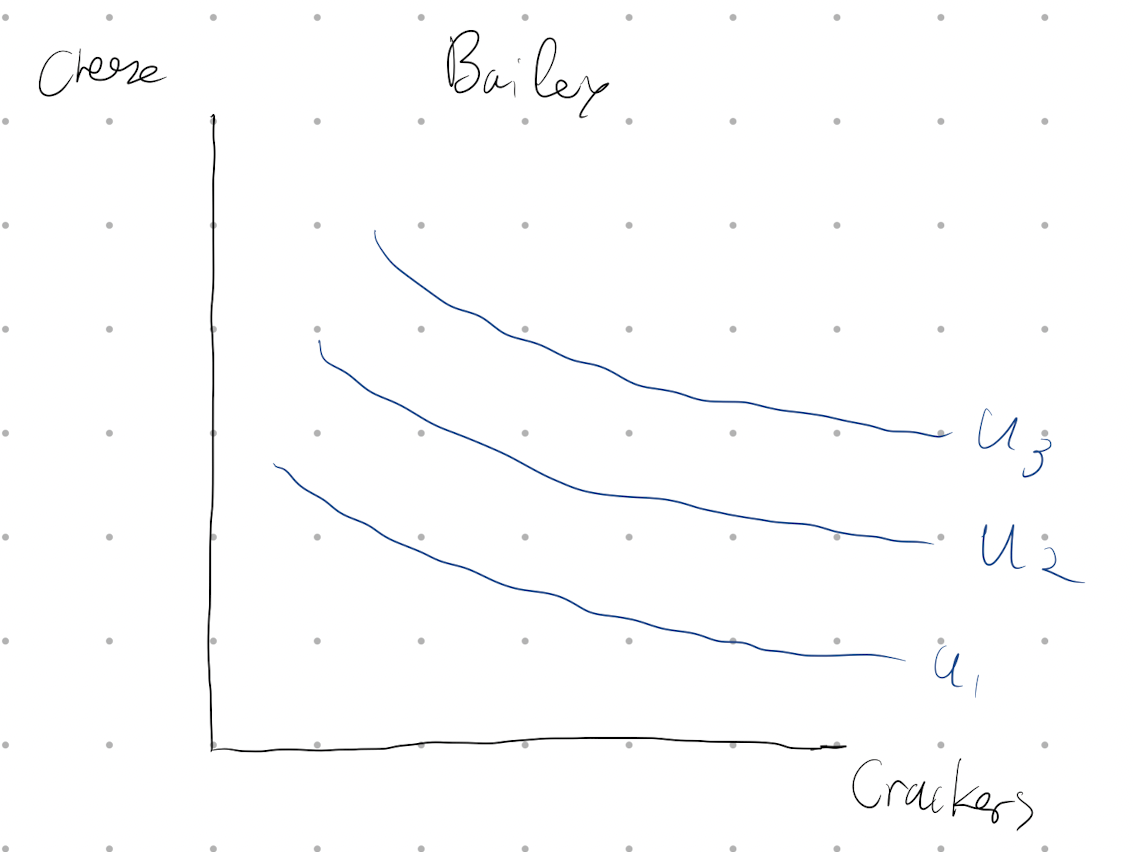
\includegraphics[width=10cm]{HW2Q12A}
\end{center}
\subsection*{Part B}
\begin{center}
	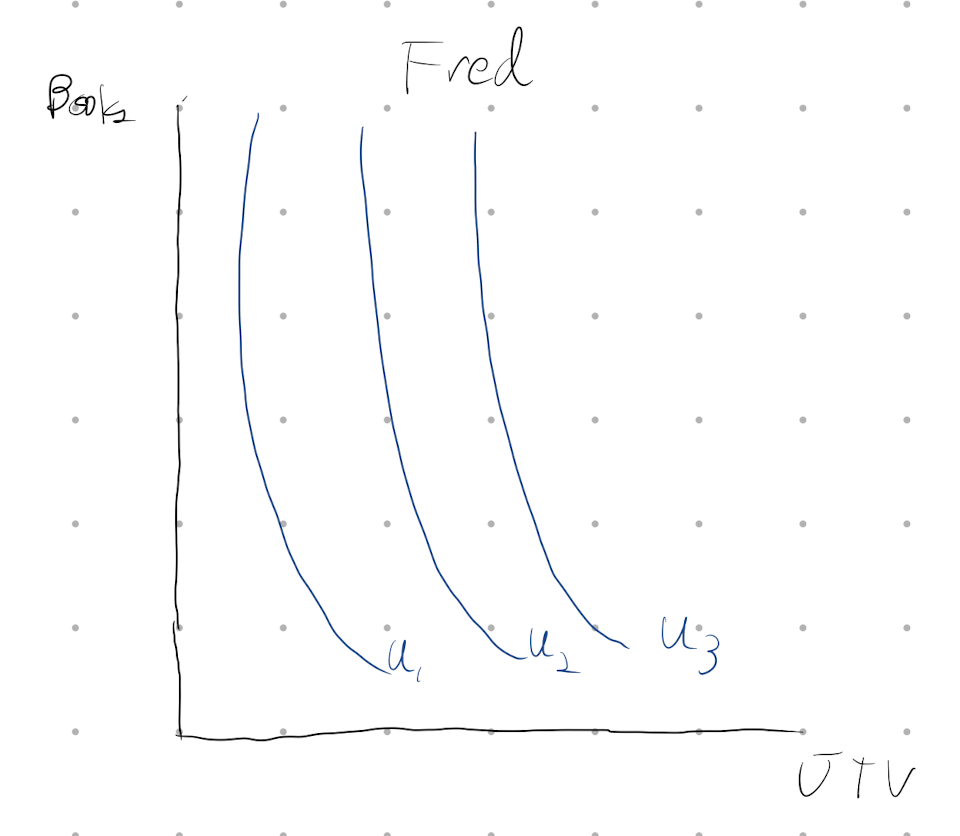
\includegraphics[width=10cm]{HW2Q12B}
\end{center}
\subsection*{Part C}
\begin{center}
	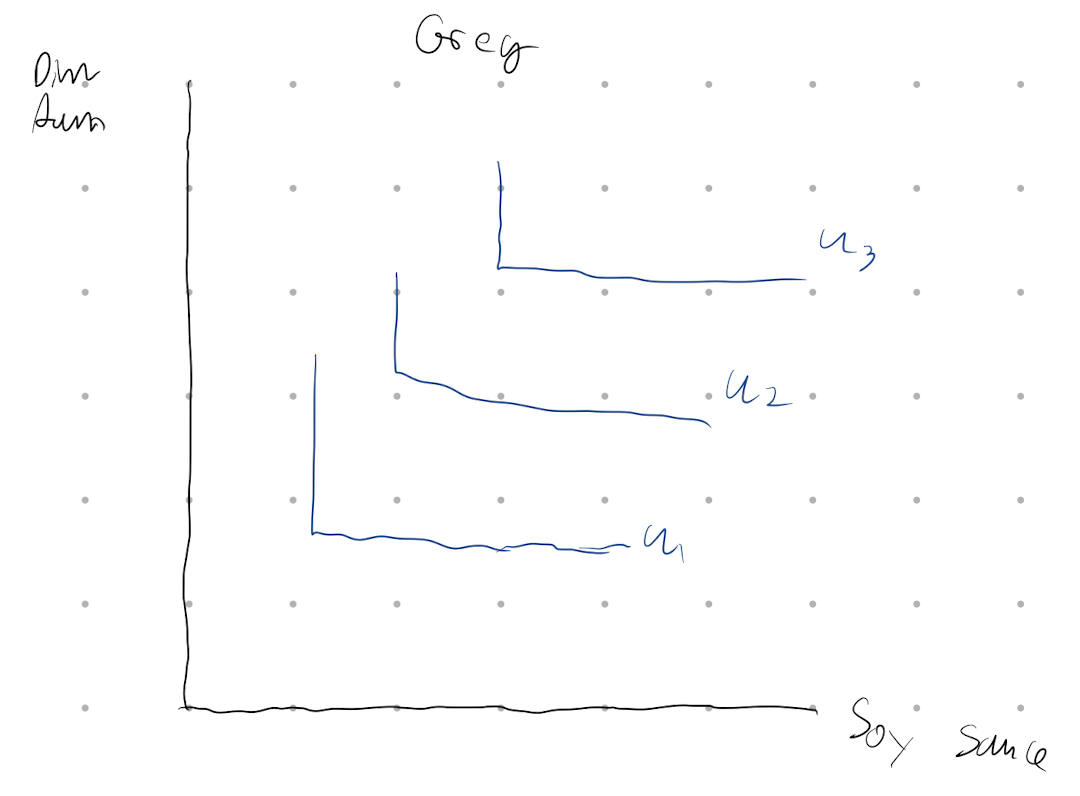
\includegraphics[width=10cm]{HW2Q12C}
\end{center}
\subsection*{Part D}
\begin{center}
	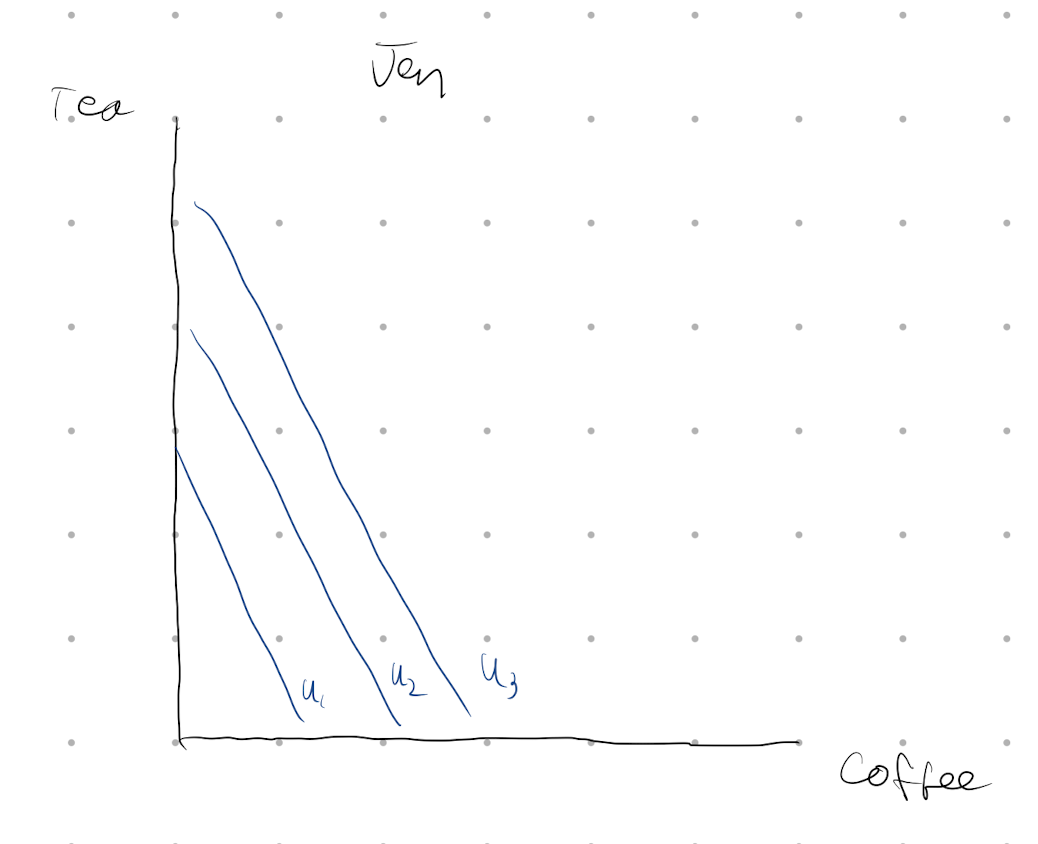
\includegraphics[width=10cm]{HW2Q12D}
\end{center}
}\end{document}